Ogni componente in Mole.io � stato realizzato cercando di rispettare il pi� possibile due concetti fondamentali, che sono stati il denominatore comune del progetto: l'estensibilit� e la flessibilit�.

Le comunicazioni tra i diversi componenti del sistema sono realizzate utilizzando il protocollo HTTP. I diversi attori si scambiano informazioni attraverso dei \textit{contratti}, le interfacce \textit{REpresentational State Transfer} (REST).

Una interfaccia REST \cite{webber2010rest} � uno stile architetturale composto da regole, ed elementi che permettono l'accesso a insiemi dati organizzati in maniera strutturata.

Nei sistemi REST, le risorse sono indirizzate secondo regole ben definite e note a priori. Immaginando di modellare una interfaccia REST che permetta l'accesso ad un sistema di utenti e di relazioni tra essi, potremmo definire i seguenti \textit{Uniform Resource Identifier} (URI) per estrarne informazioni:

\begin{itemize}
\item \verb|/users|: restituisce l'elenco di tutti gli utenti presenti nel sistema;
\item \verb|/users/marco|: restituisce i dati relativi all'utente di nome  \verb|marco|;
\item \verb|/users/marco/friends|: restituisce l'elenco degli amici di \verb|marco|;
\item \verb|/users/marco/friends/fabio|: restituisce i dati dell'utente \verb|fabio|, amico di \verb|marco|;
\end{itemize}

Come si pu� notare, � stata definita una convenzione, una regola, per ottenere i dati dal sistema e modellare le relazioni tra essi. \`{E} stata inoltre, implicitamente, generata una modalit� logica di navigazione attraverso i dati che permette di raggiungere le informazioni desiderate.

Le interfacce REST implementate in Mole.io restituiscono dati in formato JSON \cite{crockford2008javascript}. Riprendendo l'esempio precedente, si potrebbe immaginare che il sistema risponda alle richieste effettuate nell'ordine, restituendo i seguenti dati:

\begin{verbatim}
GET /users
(RISPOSTA) [ 'marco', 'fabio', 'paola', 'gianni' ]
GET /users/marco
(RISPOSTA) { name: 'marco', surname: 'bianchi', age: '25' }
GET /users/marco/friends
(RISPOSTA) [ 'fabio', 'paola' ]
GET /users/marco/friends/fabio
(RISPOSTA) { name: 'fabio', surname: 'verdi', age: '31' }
\end{verbatim}

Come � stato anticipato, le interfacce REST, utilizzano il protocollo HTTP per scambiare dati. Questo protocollo mette a disposizione diverse tipologie di messaggi, ognuna di queste si pu� immaginare come una \textit{azione} compiuta su una risorsa: quella indicata dall'\textit{endpoint} dell'interfaccia. I comandi utilizzati per dialogare con un servizio REST sono:
\begin{description}
\item[POST] permette di creare una nuova risorsa. Di solito, in caso di succeso, il servizio restituisce il dato appena creato;
\item[GET] richiede lo stato corrente di una risorsa;
\item[PUT] applica una modifica ad una risorsa esistente;
\item [DELETE] elimina una risorsa;
\end{description}

In letteratura, questa modalit� di interazione con i dati, � definita \textit{Create-Read-Update-Delete} (CRUD).

Ad esempio, volendo inserire un nuovo utente si potrebbe utilizzare la seguente richiesta:
\begin{verbatim}
POST /users 
{ name: 'guido', surname: rossi', age: '22' }
\end{verbatim}

A questo punto, � possibile verificare l'esito dell'inserimento con:
\begin{verbatim}
GET /users 
(RISPOSTA) [ 'marco', 'fabio', 'paola', 'gianni', 'guido' ]
GET /users/guido
(RISPOSTA) { name: 'guido', surname: rossi', age: '22' }
\end{verbatim}

Una delle caratteristiche di REST � l'assenza del supporto alle \textit{session}. I sistema modellati secondo queste interfacce sono, infatti,  \textit{state-less}, cio� non presentano correlazioni tra richieste successive. L'approccio adottato da REST, in questo caso, � esattamente allineato con quello adottato da HTTP, anch'esso state-less. Come anticipato nella sezione \ref{AngularJS_e_altre_tecnologie_di_frontend}, questa peculiarit� rende i framework per realizzare single-page application, i tool ideali per lavorare in tale ambito.  

Nell'architettura di Mole.io si possono individuare due \textit{layer} principali: 

\begin{description}
\item [Insertion] � la porzione di sistema che si occupa dell'inserimento dei dati provenienti dall'esterno. Questa sezione � composta, a sua volta, dai \textit{mole-contacts} e dal server \textit{mole}. La sezione \ref{mole} si occupa di descrivere i dettagli dell'architettura del layer di insertion.  
\item [Presentation] si occupa dell'estrazione dei dati dal sistema e della loro presentazione all'utente. Le componenti di questo modulo sono la \textit{user-interface} (UI) AngularJS e il server \textit{mole-suit}. Il layer di presentation verr� approfondito nella sezione \ref{mole-suit}.
\end{description}

Ogni componente ricopre un ruolo ben preciso nel sistema e comunica con gli altri attori attraverso interfacce di tipo REST. 

\begin{description}
\item [mole-contact] risiede all'interno di una applicazione detta \textit{source} e si occupa dell'invio delle informazioni da salvare (log e messaggi) al server mole;
\item [mole] il suo compito � validare le informazioni in arrivo dai diversi mole-contact e salvarle all'interno del database;
\item [user interface] � la vera e propria interfaccia grafica di Mole.io. Permette agli utenti di interagire con il sistema e dialoga direttamente con mole-suit per ottenere i dati da mostrare;
\item[mole-suit] � il server che si occupa di estrarre dal database i dati richiesti dagli utenti;
\end{description}

La figura \ref{fig:rest} rappresenta schematicamente le comunicazioni instaurate dalle diverse componenti del sistema. Come � possibile notare dal grafico, Mole.io � in grado di interagire con svariate tipologie di applicazioni (source): web, desktop oppure mobile. Nella sezione \ref{mole} verranno illustrate le interazioni tra source e mole-contact.\\

\begin{figure}[H]
\centering
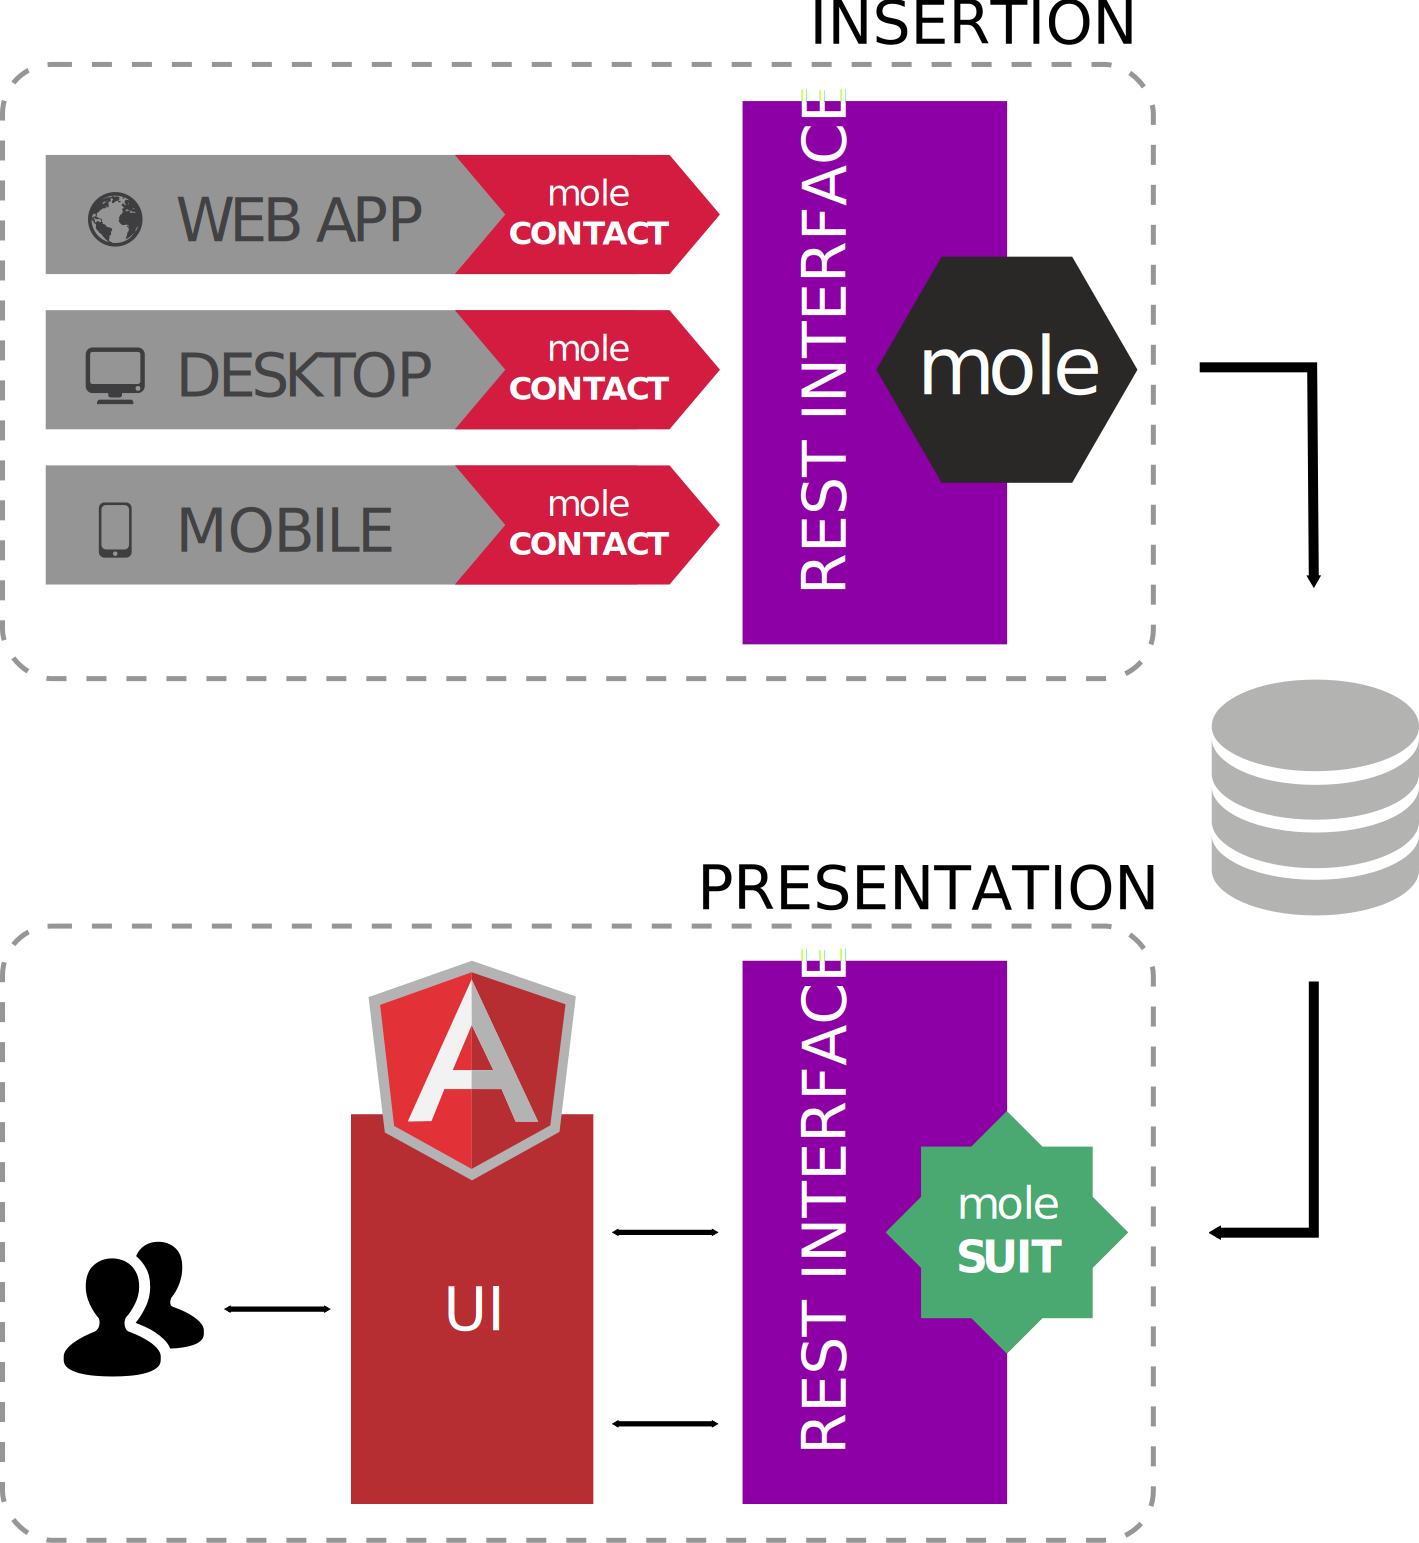
\includegraphics[width=1.0\linewidth]{./img/rest}
\caption[L'architettura di Mole.io]{L'architettura di Mole.io}
\label{fig:rest}
\end{figure}

In tabella \ref{tab:endpoint} sono riportati i principali endpoint delle interfacce REST esposte da ciascun componente in Mole.io. Per ciascun endpoint sono state riportate la tipologia di comando utilizzata per interagire con l'URI (\verb|GET| o \verb|POST|) e una descrizione delle funzionalit� offerte da esso.

\begin{table}[H]
\begin{center}
\begin{tabular}{|l|l|l|p{3.5cm}|}
\hline 
& \textbf{Tipo} & \textbf{Endpoint} & \textbf{Descrizione} \\
\hline
\multirow{3}{*}{\rotatebox[origin=c]{90}{\textbf{mole}}} & \verb|POST| & \verb|/whispers| & permette ai mole-contact di inviare whisper a mole \\
\hline
\multirow{14}{*}{\rotatebox[origin=c]{90}{\textbf{mole-suit}}} & \verb|GET| & \verb|/sources| & restituisce l'elenco delle source \\
\cline{2-4}
& \verb|POST| & \verb|/sources| & permette di inserire una nuova source \\
\cline{2-4}
& \verb|GET| & \verb|/sources/sID| & restituisce i dati della source con id \verb|sID| \\
\cline{2-4}
& \verb|GET| & \verb|/sources/sID/whispers| & restituisce l'elenco degli whisper ricevuti dalla source con id \verb|sID| \\
\cline{2-4}
& \verb|GET| & \verb|/sources/sID/whispers/wID| & restituisce l'elenco al whisper con id \verb|wID| ricevuto dalla source con id \verb|sID| \\
\hline
\end{tabular}
\caption{I principali endpoint REST forniti da Mole.io}\label{tab:endpoint}
\end{center}
\end{table}

Implementare una interfaccia REST con Node.js � piuttosto semplice, specialmente se si utilizza il modulo Express, descritto nella sezione \ref{Npm_e_moduli}. Express, infatti, mette a disposizione dello sviluppatore un sistema molto potente di \textit{route}, che permettono di identificare la risorsa desiderata a fronte di una richiesta in arrivo. Il codice seguente implementa un esempio di rotta con Express.\\

\begin{verbatim}
var express = require('express');
var app = express();
app.use(app.router);
app.get('/now', function(req, res) {
  res.json({ now: new Date().toString() });
});
\end{verbatim}

L'applicazione Node.js carica il modulo Express e genera una applicazione utilizzando tale modulo. Successivamente viene registrata una rotta che corrisponde all'URI \verb|/now|. All'arrivo di una richiesta di tipo \verb|GET| verso la risorsa \verb|/now|, Express esegue la callback associata e restituisce un documento JSON simile a quello seguente.
\begin{verbatim}
{ "now": "Sun Mar 09 2014 20:48:35 GMT+0100 (CET)" }
\end{verbatim}

Il \textit{router} Express, come molti altri plugin di questo sistema, rappresenta un \textit{middleware}. Il comando \verb|app.use(app.router);|, infatti, indica ad Express di utilizzare il middleware \verb|router| per filtrare le richieste in arrivo.

Un middleware � un modulo software che filtra ogni richiesta in arrivo dai client. I middleware cooperano tra loro e vengono attivati in successione. Il flusso di lavoro di un middleware � riassumibile in tre fasi principali:

\begin{enumerate}
\item ottenere la richiesta;
\item validare la richiesta ed eseguire funzionalit� specifiche associate al middleware stesso;
\item passare la richiesta al prossimo middleware;
\end{enumerate}

Seguendo il medesimo schema di funzionamento, i middleware, elaborano le risposte provenienti dall'applicazione e restituite al client. La figura \ref{fig:middleware} illustra il funzionamento di questo sistema.

\begin{figure}[H]
\centering
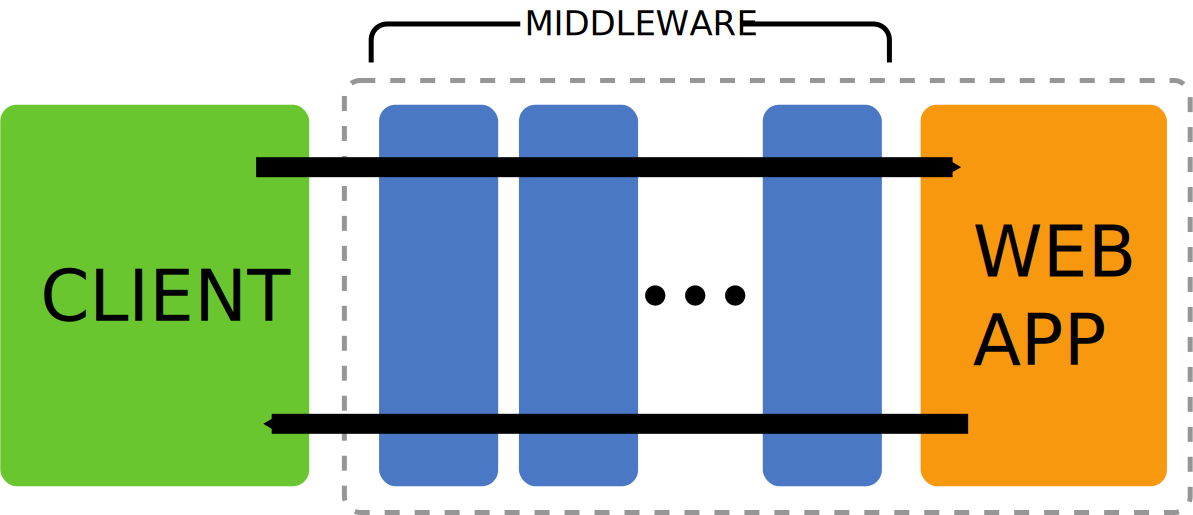
\includegraphics[width=1.0\linewidth]{./img/middleware}
\caption[Schema di funzionamento dei middleware]{Schema di funzionamento dei middleware}
\label{fig:middleware}
\end{figure}

%Nell'architettura di Mole.io si possono innanzitutto individuare quattro macro-componenti principali: \textit{mole-contact}, \textit{mole}, \textit{mole-suit} e il frontend o \textit{user-interface} (UI). Nella sezione \ref{Moleio} sono stati introdotti alcuni di questi attori, definendo la genesi dei rispettivi nomi. I componenti mole e mole-suit, sono server web realizzati in Node.js e utilizzano interfacce di tipo REST per comunicare con i client, rispettivamente i mole-contact e la UI.
%La tabella \ref{tab:endpoint}, introduce un nuovo concetto: le \textit{source}. Una source �, come suggerisce il nome, una sorgente di informazioni per Mole.io o, per meglio identificare il ruolo della source, una sorgente di whisper.
%Secondo la nomenclatura adottata in Mole.io, una source � infatti una applicazione contenente un mole-contact. Mole.io � in grado di interagire con svariate tipologie di applicazioni: web, desktop oppure mobile. L'unico requisito necessario � la possibilit� di utilizzare comunicazioni di rete per permettere al mole-contact di contattare il server mole. 
%Questo \textit{layer} dell'applicazione si occupa dell'inserimento dei dati nel sistema e si avvale di diversi moduli per fare in modo che gli whisper vengano salvati, aggregati e organizzati nel database.
%Nello schema \ref{} � riportata l'architettura del layer di insertion, essa � composta da diversi moduli:
%mole-contacts
%la porzione di sistema che si occupa dell'inserimento dei dati provenienti dall'esterno, � composta a sua volta dai \textit{mole-contacts}, da \textit{mole} e dai \textit{denormalizers}.
